\chapter{ComStock Outputs}
ComStock creates a wide array of data that can be analyzed and aggregated to draw conclusions. While it is common to look at how results vary by building type and climate zone, ComStock provides a wide range of outputs not traditionally provided in large-scale analyses, with the hope of providing maximum utility.

Sections \ref{rawsimulationresults} and \ref{dataviewer} describe how to access ComStock outputs. Additionally, the sample building energy models are available at \url{https://data.openei.org/} in the nrel-pds-building-stock data lake. See the README.md file for details.

\section{Energy Consumption by Fuel and End Use}
ComStock provides energy consumption by fuel and end use at both an annual and time-series (typically 15-minute time steps for one year) resolution. Not all combinations of fuels and end uses are found in ComStock. The definitions below describe the fuels and end uses in detail.

ComStock provides modeled energy consumption for the following \textbf{fuels}:

\begin{itemize}
  \item \textbf{Electricity}: This represents the electricity that is delivered to the building through the power grid and consumed on-site. How this electricity is generated depends on the generation mix found on the power grid in the region serving the building. This does not include electricity that is generated through a backup generator.
  \item \textbf{Natural Gas}: This represents the natural gas that is delivered to the building through the natural gas pipeline system and consumed on-site.
  \item \textbf{Propane}: This represents the propane that is delivered to the building in tanks and consumed on-site.
  \item \textbf{Fuel Oil}: This represents the liquid fuel oil that is delivered to the building, stored in tanks, and consumed on-site.
  \item \textbf{Other Fuel}: In some ComStock outputs, propane and fuel oil are combined and reported together as ``other fuel'' due to reporting limitations in the simulation engine. Where this is the case, propane and fuel oil are not reported separately to avoid double-counting.
  \item \textbf{District Heating}: This represents the hot water or steam that is delivered to the building through a district heating piping system and consumed on-site. The quantity of energy consumed represents only the energy extracted from the district heating system by the building; it does not represent the consumption of electricity or natural gas at the district heating plant required to provide heat to the building. In order to capture the energy consumption of the district heating plant, assumptions about distribution heat losses, pumping power, and district heating plant equipment efficiency and controls may be made.
  \item \textbf{District Cooling}: This represents the chilled water that is delivered to the building through a district cooling piping system and consumed on-site. The quantity of energy consumed represents only the energy extracted from the district cooling system by the building; it does not represent the consumption of electricity or natural gas at the district cooling plant required to provide chilled water to the building. In order to capture the energy consumption of the district cooling plant, assumptions about distribution heat gains, pumping power, and district cooling plant equipment efficiency and controls may be made.
\end{itemize}

ComStock provides modeled energy consumption for the following \textbf{end uses} for each applicable fuel:

\begin{itemize}
\item \textbf{Cooling}: This includes all energy consumed by primary cooling equipment such as chillers, direct expansion air conditioners (includes condenser fan energy), and direct expansion heat pumps in cooling mode (includes condenser fan energy). This also includes parasitic energy consumption of the equipment, such as pan heaters, defrost energy, and any energy needed to overcome modeled pipe losses.
\item \textbf{Heating}: This represents all energy consumed by primary heating equipment such as boilers, furnaces, natural gas heating coils, electric resistance strip heating coils, and direct expansion heat pumps in heating mode (includes evaporator fan energy). This also includes parasitic energy consumption of the equipment, such as pilot lights, standby losses, defrost energy, and any energy needed to overcome modeled pipe losses.
\item \textbf{Fans}: This includes all energy consumed by supply fans, return fans, exhaust fans, and kitchen hoods in the building. It excludes the condenser fan energy from direct expansion coils, which is captured in cooling and heating, as described above.
\item \textbf{Pumps}: This includes all energy consumed by pumps for the purpose of moving hot water for heating and service water heating, chilled water for cooling, and condenser water for heat rejection.
\item \textbf{Heat Recovery}: This includes the energy used to turn heat or enthalpy wheels, plus the increased fan energy associated with the increased pressure rise caused by the heat recovery wheels.
\item \textbf{Heat Rejection}: This includes the energy used to run cooling towers and fluid coolers to reject heat from the condenser water loop to the air. As previously noted, condenser fans on direct expansion cooling and heating coils are included in heating and cooling.
\item \textbf{Humidification}: This includes all energy used to purposely increase humidity in the building. Most buildings are assumed not to use humidification.
\item \textbf{Water Systems}: This includes all energy consumed by the primary service hot water supply equipment, such as boilers and water heaters. This also includes parasitic energy consumption of the equipment, such as pilot lights, standby losses, and any energy needed to overcome modeled pipe losses.
\item \textbf{Refrigeration}: This includes all energy used by large refrigeration cases and walk-ins such as those commonly found in grocery stores and large commercial kitchens. Plug-in refrigerators, such as those commonly found in the checkout areas of retail stores, are included in interior equipment.
\item \textbf{Interior Lighting}: This includes all energy used to light the interior of the building, including general lighting, task lighting, accent lighting, and exit lighting.
\item \textbf{Exterior Lighting}: This includes all energy used to light the exterior of the building and the surrounding area, including parking lot lighting, entryway illumination, and wall washing.
\item \textbf{Interior Equipment}: This includes all energy used in the building that was not included in one of the other categories. This covers miscellaneous electric loads such as computers and monitors, large equipment such as elevators, and special-purpose equipment such as data center and IT-closet servers. This is a large and coarse bin, largely because the variety of energy-consuming devices found in buildings is large and little comprehensive data are available.
\end{itemize}

\begin{figure}
    \centering
    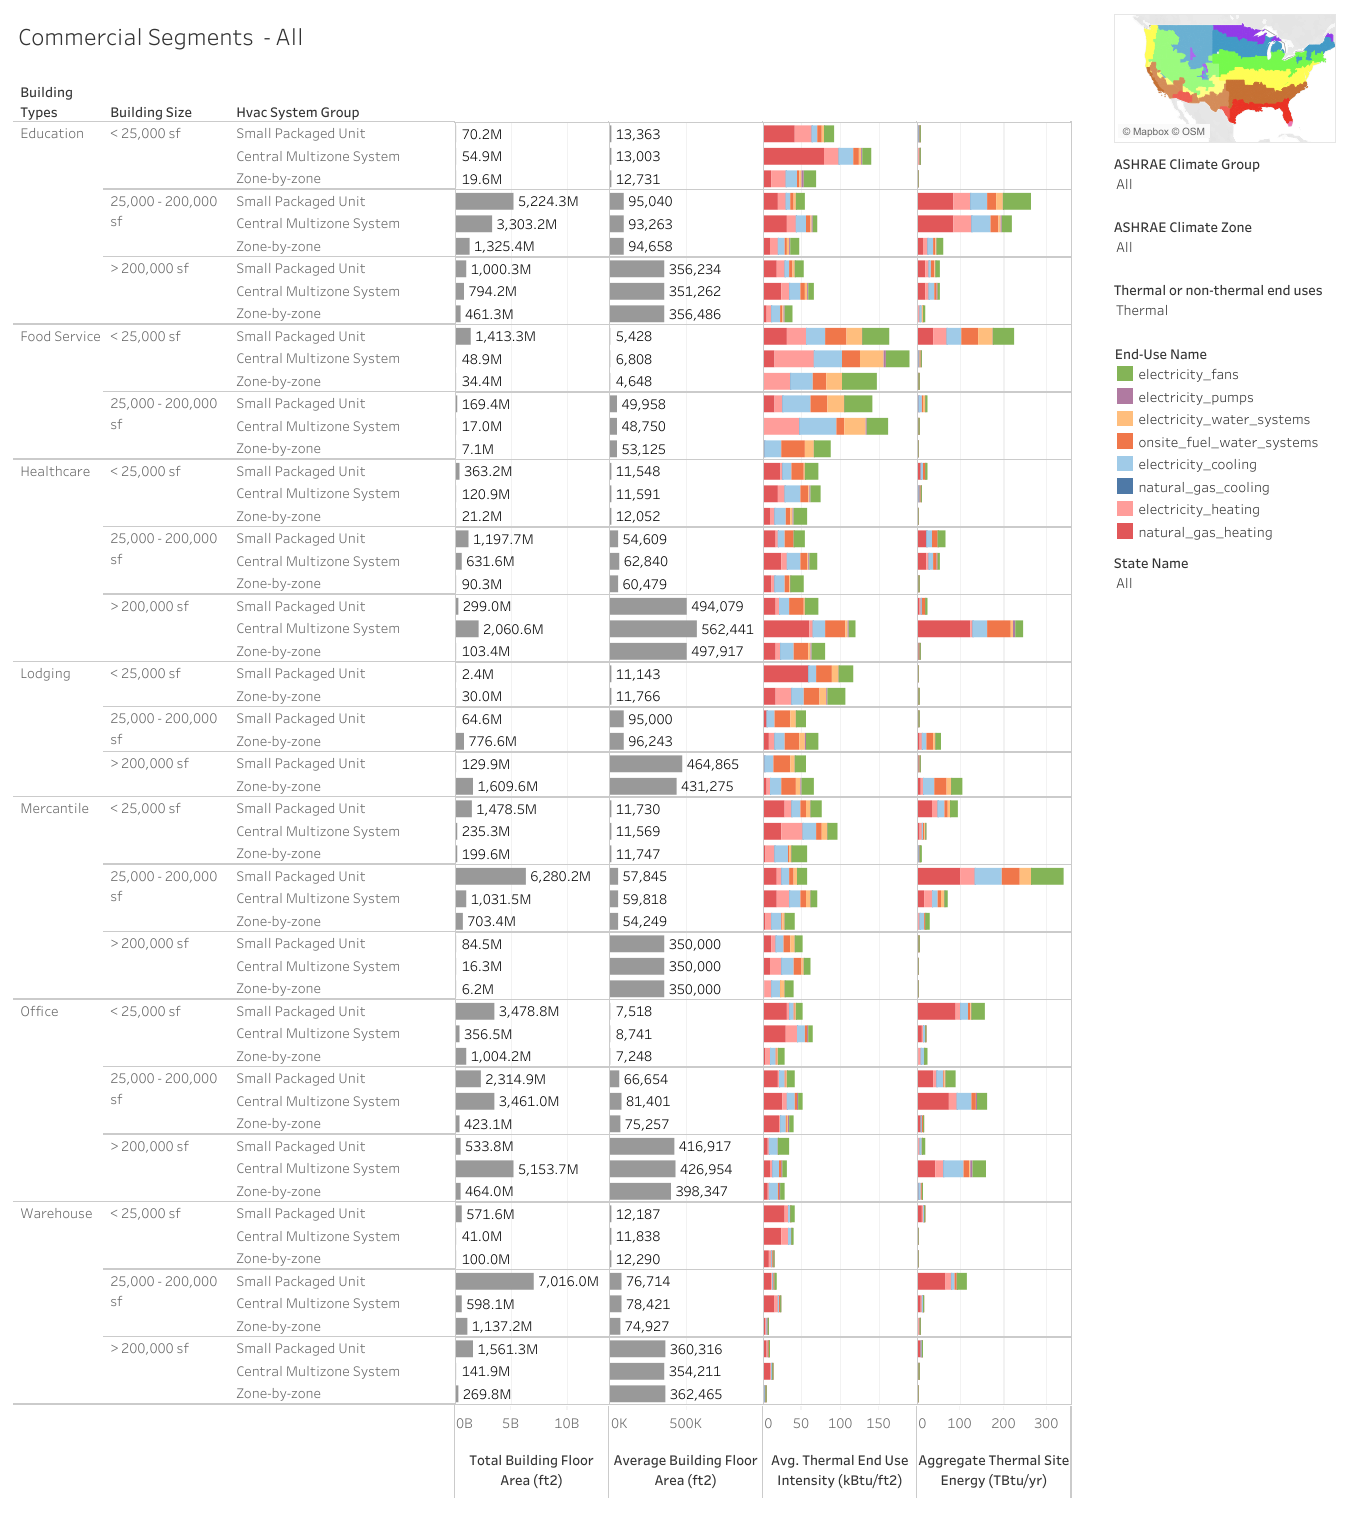
\includegraphics
    [width=\textwidth]{figures/Segments_typology.png}
    \caption[Example of ComStock Results]{Example ComStock Results}
    \label{fig:segments_typology}
\end{figure}

\section{Building Characteristics}
In addition to energy consumption data, ComStock outputs include a variety of building input characteristics. Most of these are either direct or indirect inputs to the building model generation workflow. Units for these characteristics are described in the files that accompany the ComStock data sets. Names and descriptions for these characteristics are included in Table \ref{tab:building_input_characteristics}.

\begin{center}
\small
\begin{longtable}{|p{3in}|p{3in}|}
\caption{Building Input Characteristics} \\ \hline
\label{tab:building_input_characteristics}
\textbf{Building Input Characteristic} & \textbf{Description} \\ \hline
\endfirsthead
\multicolumn{2}{c} {{\bfseries \textit{Continued from previous page}}} \\ \hline
\textbf{Building Input Characteristic} & \textbf{Description} \\ \hline
\endhead
in.year\_built                                                                   & Year of original building construction                                                                                                                               \\ \hline
in.building\_id                                                                  & ID number for model                                                                                                                                                  \\ \hline
in.upgrade\_id                                                                   & ID of upgrade, including 00 for baseline                                                                                                                              \\ \hline
in.upgrade\_name                                                                 & Name of upgrade (if an upgrade was run)                                                                                                                                \\ \hline
in.tstat\_clg\_delta\_f                                                          & Cooling thermostat unoccupied set point temperature delta from primary occupied cooling set point. A value of 999 indicates that default values were used for the model      \\ \hline
in.tstat\_clg\_sp\_f                                                             & Cooling thermostat occupied set point. A value of 999 indicates that default values were used for the model                                                                  \\ \hline
in.tstat\_htg\_delta\_f                                                          & Heating thermostat unoccupied set point temperature delta from primary occupied heating set point. A value of 999 indicates that default values were used for the model     \\ \hline
in.tstat\_htg\_sp\_f                                                             & Heating thermostat occupied set point. A value of 999 indicates that default values were used for the model                                                                  \\ \hline
in.aspect\_ratio                                                                 & Aspect ratio of building geometry, which is the ratio of the north/south facade length relative to the east/west facade length                                                \\ \hline
in.window\_type                                                                  & Type of windows in the model                                                                                                                                         \\ \hline
in.building\_subtype                                                             & Building subtype of the model                                                                                                                                            \\ \hline
in.county                                                                        & County ID of the building model                                                                                                                                          \\ \hline
in.comstock\_building\_type                                                      & Primary building type of the model                                                                                                                                       \\ \hline
in.rotation                                                                      & Building rotation off of north axis (positive value is clockwise)                                                                                                    \\ \hline
in.number\_of\_stories                                                           & Building number of stories above grade                                                                                                                               \\ \hline
in.floor\_area                                                                   & Building total floor area                                                                                                                                            \\ \hline
in.hvac\_system\_type                                                            & Building  primary HVAC system type                                                                                                                                   \\ \hline
in.wall\_construction\_type                                                      & Type of construction used for exterior walls                                                                                                                     \\ \hline
in.weekday\_operating\_hours                                                     & Building duration of weekday hours of operation, which influences the duration of schedules                                                                               \\ \hline
in.weekday\_opening\_time                                                        & Building weekday start hour, which impacts the start time of schedules                                                                                                \\ \hline
in.weekend\_operating\_hours                                                     & Building duration of weekend hours of operation, which influences the duration of schedules                                                                               \\ \hline
in.weekend\_opening\_time                                                        & Building weekend start hour, which impacts the start time of schedules                                                                                                \\ \hline
in.energy\_code\_followed\_during\_last\_exterior\_lighting\_replacement         & Specifies the energy code used to determine exterior lighting power and controls                                                                                     \\ \hline
in.energy\_code\_followed\_during\_last\_hvac\_replacement                       & Specifies the energy code used to determine HVAC system types, efficiencies, and controls                                                                            \\ \hline
in.energy\_code\_followed\_during\_last\_interior\_equipment\_replacement        & Specifies the energy code used to determine interior equipment loads                                                                                                 \\ \hline
in.energy\_code\_followed\_during\_last\_roof\_replacement                       & Specifies the energy code used to determine roof insulation values                                                                                                   \\ \hline
in.energy\_code\_followed\_during\_last\_service\_water\_heating\_replacement    & Specifies the energy code used to determine service water heating efficiencies                                                                                       \\ \hline
in.energy\_code\_followed\_during\_last\_walls\_replacement                      & Specifies the energy code used to determine wall insulation values                                                                                                   \\ \hline
in.energy\_code\_followed\_during\_original\_building\_construction              & Specifies the date of construction of the modeled building, which impacts the assumed energy code year of building subsystems                                          \\ \hline
in.heating\_fuel                                                                 & Building primary HVAC heating fuel source                                                                                                                            \\ \hline
in.hvac\_night\_variability                                                      & Specifies the nighttime HVAC operation used in the model, which impacts fan and ventilation behavior during unoccupied times                                       \\ \hline
in.interior\_lighting\_generation                                                & The technology used for interior lighting in the building                                                                                                            \\ \hline
in.number\_stories                                                               & Specifies the number of stories of the building                                                                                                                      \\ \hline
in.floor\_area\_category                                                         & Specifies the rentable area range of the building                                                                                                                    \\ \hline
in.service\_water\_heating\_fuel                                                 & Building primary service water heating fuel source                                                                                                                   \\ \hline
in.nhgis\_tract\_gisjoin                                                         & Census tract identifier in \href{https://www.nhgis.org/geographic-crosswalks\#details}{National Historical Geographic Information System (NHGIS) format}                                                                 \\ \hline
in.nhgis\_county\_gisjoin                                                        & County identified in \href{https://www.nhgis.org/geographic-crosswalks\#details}{NHGIS format}                                                                       \\ \hline
in.state\_name                                                                   & Full name of state                                                                                                                                                   \\ \hline
in.state\_abbreviation                                                           & Postal abbreviation of state                                                                                                                                         \\ \hline
in.census\_division\_name                                                        & Census division name                                                                                                                                                 \\ \hline
in.census\_region\_name                                                          & Census region name                                                                                                                                                   \\ \hline
in.weather\_file\_2018                                                           & Weather file used for the 2018 AMY simulations                                                                                                                       \\ \hline
in.weather\_file\_TMY3                                                           & Weather file used for the TMY3 simulations                                                                                                                           \\ \hline
in.climate\_zone\_building\_america                                              & DOE Building America climate zone                                                                                                                                    \\ \hline
in.climate\_zone\_ashrae\_2006                                                   & ASHRAE Standard 169--2006                                                                                                                                                 \\ \hline
in.iso\_region                                                                   & Electric system independent system operator/regional transmission organization (ISO/RTO) region                                                                                                                                       \\ \hline
in.reeds\_balancing\_area                                                        & Balancing area ID for the NREL Regional Energy Deployment System (ReEDS) modeling tool                                                                                                                   \\ \hline
in.resstock\_county\_id                                                          & State abbreviation and county name                                                                                                                                   \\ \hline
in.nhgis\_puma\_gisjoin                                                          & Census PUMA identifier in \href{https://www.nhgis.org/geographic-crosswalks\#details}{NHGIS format}                                                                  \\ \hline
in.ejscreen\_census\_tract\_percentile\_for\_people\_of\_color                   & Percentile for \% people of color in building's census tract. See \href{https://www.epa.gov/ejscreen}{U.S. Environmental Protection Agency (EPA) Environmental Justice Screening and Mapping Tool (EJSCREEN) documentation} for details                       \\ \hline
in.ejscreen\_census\_tract\_percentile\_for\_low\_income                         & Percentile for \% low-income in building's census tract. See \href{https://www.epa.gov/ejscreen}{EPA EJSCREEN documentation} for details                            \\ \hline
in.ejscreen\_census\_tract\_percentile\_for\_less\_than\_high\_school\_education & Percentile for \% less than high school in building's census tract. See \href{https://www.epa.gov/ejscreen}{EPA EJSCREEN documentation} for details                 \\ \hline
in.ejscreen\_census\_tract\_percentile\_for\_people\_in\_linguistic\_isolation   & Percentile for \% of individuals in linguistic isolation in building's census tract. See \href{https://www.epa.gov/ejscreen}{EPA EJSCREEN documentation} for details.\\ \hline
in.ejscreen\_census\_tract\_percentile\_percent\_people\_under\_5                & Percentile for \% under age 5 in building's census tract. See \href{https://www.epa.gov/ejscreen}{EPA EJSCREEN documentation} for details                          \\ \hline
in.ejscreen\_census\_tract\_percentile\_for\_people\_over\_64                    & Percentile for \% over age 64 in building's census tract. See \href{https://www.epa.gov/ejscreen}{EPA EJSCREEN documentation} for details                           \\ \hline
in.ejscreen\_census\_tract\_percentile\_for\_demographic\_index                  & Percentile for demographic index in building's census tract. See \href{https://www.epa.gov/ejscreen}{EPA EJSCREEN documentation} for details                        \\ \hline
in.cejst\_is\_disadvantaged                                                      & Whether the building's census tract is identified as a disadvantaged community in the EPA Climate and Economic Justice Screening Tool (CEJST). See \href{https://screeningtool.geoplatform.gov/en/methodology}{CEJST documentation} for more details                      \\ \hline
\end{longtable}
\end{center}
\pagebreak
\section{Building Summary Statistics}
In addition to the building input characteristics, ComStock outputs include a variety of summary statistic information about the building.  These statistics captures building characteristics that result from the complex rules that are applied to HVAC systems after sizing routines and are therefore not easy to discern from the building input characteristics. Units for these outputs are described in the files that accompany the ComStock data sets. Names and descriptions for these summary statistics are included in Table \ref{tab:building_summary_stats}

\section{Greenhouse Gas Emissions Reporting}
ComStock calculates the greenhouse gas emissions from the building stock and savings from measures using both historical and projected emissions data.

\subsection{Electricity Emissions}
\subsubsection{eGRID Historical Emissions}
Historical emissions use the CO\textsubscript{2}-equivalent total output emission rate from EPA's Emissions and Generation Resource Integrated Database (eGRID)\citep{egrid2020}. ComStock results include the historical emissions for 2018, 2019, 2020, and 2021 using eGRID U.S. state and eGRID subregion emissions factors. eGRID regions are similar to Cambium grid regions but not identical. Notably, eGrid separates out New York into upstate, New York City, and Long Island. Cambium uses a whole-state average, and historical emissions use the New York state average instead of the grid region for New York buildings. Historical eGrid emissions rates are an \textit{annual} average multiplied by the total annual electricity use.

\subsubsection{Cambium Projected Emissions}
Projected emissions use data from NREL's Cambium 2022 data set \citep{cambium2022}. Projected emissions consider both the average emissions rate (AER) and the long-run marginal emission rate (LRMER).  LRMER, described in \cite{GAGNON2022103915}, is an estimate of the rate of emissions that would be either induced or avoided by a long-term (i.e., more than several years) change in electrical demand.  LRMER data is levelized over 15 and 30 years\citep{cambium2022}. ComStock results including End Use Savings Shapes round 1 results and earlier projects used emissions factors from the Cambium 2021 data \citep{cambium2021},\citep{lrmer_data2022}.

\subsection{On Site Fossil Fuel Emissions}
Natural gas, propane, and fuel oil emissions use the emission factors in \textit{Table 5.1.2(1) National Average Emission Factors for Household Fuels} defined in \textit{ANSI/RESNET/ICCC 301 Standard for the Calculation and Labeling of the Energy Performance of Dwelling and Sleeping Units using an Energy Rating Index}. Natural gas emissions include both combustion and pre-combustion emissions (e.g., methane leakage for natural gas).

\subsection{District Energy Emissions}
ComStock currently does not model emissions from district energy systems, as there is considerable variation by location and type of district system.